
\documentclass{beamer}
\mode<presentation>
\usepackage{amsmath}
\usepackage{amssymb}
%\usepackage{advdate}
\usepackage{graphicx}
\graphicspath{{../figs/}}
\usepackage{adjustbox}
\usepackage{subcaption}
\usepackage{enumitem}
\usepackage{multicol}
\usepackage{mathtools}
\usepackage{listings}
\usepackage{url}
\def\UrlBreaks{\do\/\do-}
\usetheme{Boadilla}
\usecolortheme{lily}
\setbeamertemplate{footline}
{
  \leavevmode%
  \hbox{%
  \begin{beamercolorbox}[wd=\paperwidth,ht=2.25ex,dp=1ex,right]{author in head/foot}%
    \insertframenumber{} / \inserttotalframenumber\hspace*{2ex} 
  \end{beamercolorbox}}%
  \vskip0pt%
}
\setbeamertemplate{navigation symbols}{}
\let\solution\relax
\usepackage{gvv}
\lstset{
%language=C,
frame=single, 
breaklines=true,
columns=fullflexible
}

\numberwithin{equation}{section}
\title{8.2.35}
\author{AI25BTECH11001 - ABHISEK MOHAPATRA}
% \maketitle
% \newpage
% \bigskip
\begin{document}
{\let\newpage\relax\maketitle}
\renewcommand{\thefigure}{\theenumi}
\renewcommand{\thetable}{\theenumi}





	 	\textbf{Question}:
foci (3, 0), a = 4.

		\textbf{Solution:}
		Given 2 foci exist for this conic,so it must be an ellipse or a hyperbola.
\begin{align}
		\therefore \vec{F_1} =\myvec{3\\0}, \vec{F_2} =\myvec{-3\\0}
\end{align}
\begin{align}
		\vec{u} = \frac{\vec{F_1}+\vec{F_2}}{2} = \myvec{0\\0}
\end{align}
\begin{align}
		\vec{n} \equiv \vec{F_1} - \vec{F_2} \equiv \myvec{1\\0}
\end{align}

Using (3) in (8.1.2.2),

\begin{align}
		\vec{V} = \myvec{1-e^2 & 0 \\ 0 & 1}
\end{align}

Given, the length of the semi-major axis

\begin{align}
		4 = \sqrt{\frac{|f|}{|1-e^2|}}
\end{align}


From (8.1.3.3), substituting from (1) and (3),

\begin{align}
\pm c e^2 = 3
\end{align}

Substituting all known values in (8.1.3.2),

\begin{align}
c = \pm \frac{1}{e} \sqrt{\frac{|f|}{|e^2-1|}}
\end{align}

In (5)-(7), there are 3 unknowns, $(c, f, e)$. Upon solving, we get  

\begin{align}
e = \frac{3}{4}, 
\quad c = \pm \frac{16}{3}, 
\quad |f| = 7.
\end{align}

Let 
\begin{align}
		\vec{x} = \myvec{ \alpha\\0}
\end{align}
be a vertex of the conic on the major axis. Substituting in (8.1.2.1),

\begin{align}
\alpha^2 + f = 0 \quad \Longrightarrow \quad f < 0
\end{align}

or,  
\begin{align}
f = -7.
\end{align}

Thus, the desired equation of the conic is  

\begin{align}
		\vec{x}^\top 
\myvec{
\frac{7}{16} & 0 \\ 
0 & 1
} 
		\vec{x} - 7 = 0
\end{align}

	Graph:
\begin{figure}[h!]
	\centering
	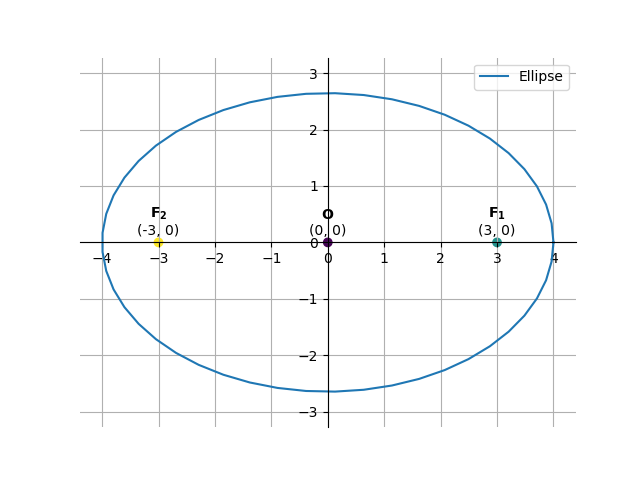
\includegraphics[width=0.7\linewidth]{img.png}
\end{figure}
\end{document}



